\documentclass[11pt]{article}
\usepackage{graphicx}
\usepackage{amssymb}
\usepackage{amsmath}
\usepackage{natbib}
\usepackage[colorlinks=true, citecolor=blue]{hyperref}
\graphicspath{{../resources/}}

\title{Notes on Boldrin and Levine}
\author{Caleb Floyd and Tom Augspurger}
\date{\today}
\begin{document}
\maketitle

\section{Summary}
\label{sec:summary}
  A simple model of innovation under perfect competition predicts that no firm will innovate, unless they are able to extract monopoly rents after the invention (e.g. via a patent).  This holds even if the innovation process is deterministic.  Without some way to earn monopoly rents (no patents) a firm will sell at marginal cost before and after the innovation.  The marginal cost will be lower after innovation, but the \emph{operating} profit will still be zero.  So a fixed cost of innovation is not worth it. 

  \cite{boldrin_levine:08:pci} construct a model where innovation does occur under perfect competition.  They mention the importance of supply constraints in generating a wedge between price and marginal cost.  I think that comes up as a condition in at least the first couple models.

\section{Assumptions}
\label{sec:assumptions}
  \begin{itemize}
    \item \textbf{Perfect competition once innovation is sold.}
  \end{itemize}

\section{Models}
\label{sec:models}
 
\subsection{Seed 24/7}
\label{sub:seed_24_7}

  Competitive rents are determined by speed of reproduction and elasticity of demand.  This market is \emph{isolated} (undefined, but I think sole inventor and didn't exist before invention).  

  Fixed cost $C$ to innovate.  Deterministically produces tree which bears fruit (from date zero).  Each fruit grows into a tree and also bears fruit.  This links the sale of product with competition.  Supply is increase by $\beta k_t$ each period.  \emph{Price is proportional to marginal utility}.

  Supply and consumption of fruit growing at exponential rate $k_t = \beta^t$ which yields a present discounted value of revenue stream from renting trees: 
  \begin{equation} \label{eq:24_7_profit}
    q_0 = \sum_{t=0}^{\infty} (\beta \delta)^t u'(\beta^t)  
  \end{equation}
  
  where $\delta < 1$ is the consumers discount factor.  So this should be the price a producer should be willing to trade for the date-zero tree.  Which it seems to be.  She earns the consumer's marginal utility when the \emph{total} supply of fruit / trees is $\beta$.

\subsection{Seed General}
\label{sub:seed_general}

  Quite a few things change from the first model.  Drop (but still allow for) the assumption that $\beta$ > 1.  Also make the consumer's preferences depend on (consumption, labor).  Splits capital use into production of consumption goods or production of more capital.\\
  
  \textsc{Preferences:}
  \begin{equation} \label{eq:general_preferences}
     \sum_t^\infty \delta^t [u(c_t) - wL_t]
  \end{equation}
    
  It's a bit odd seeing the wage entering $U$ directly, but assume that is is forever fixed so there aren't any absurd comparative statics.\\

  \textsc{Production:} As mentioned above, production is a function of labor and capital, and is split into production of a consumption good and production of capital.

  \begin{flalign} \label{eq:general_tech}
    & c_t = F(k_t^c, l_t^c)\\
    & x_t = G(k_t^k, l_t^k)\\
    & k_{t+1} = \beta k_t + x_t \ \ \ \ \ \ \ \ \ \ \beta > 0
  \end{flalign}
  
  \textsc{Equilibrium}: ``In each period [...] equilibrium solves two maximization problems (p. 439)'', is unclear about just who is maximizing what.  Presumably we start with the firm since we're taking $k_t, L_t$ and $x_t$ as given, and allocating $k_t$ over $k_t^c, k_t^k$.
  

  \begin{align}
    &\max_{k^c_t, l^c_t}  \ \ \ c_t\\
    &st. \ \ \ \ 0 \leq c_t \leq F(k_t^c, l_t^c)\\
    & \ \ \ \, \ \ \ \ 0 \leq x_t \leq F(k_t - k_t^c, L_t - l_t^c)
  \end{align}

  PPF: $c_t = T(k_t, x_t, L_t)$ Should be $l^c_t$?
  \begin{center}
    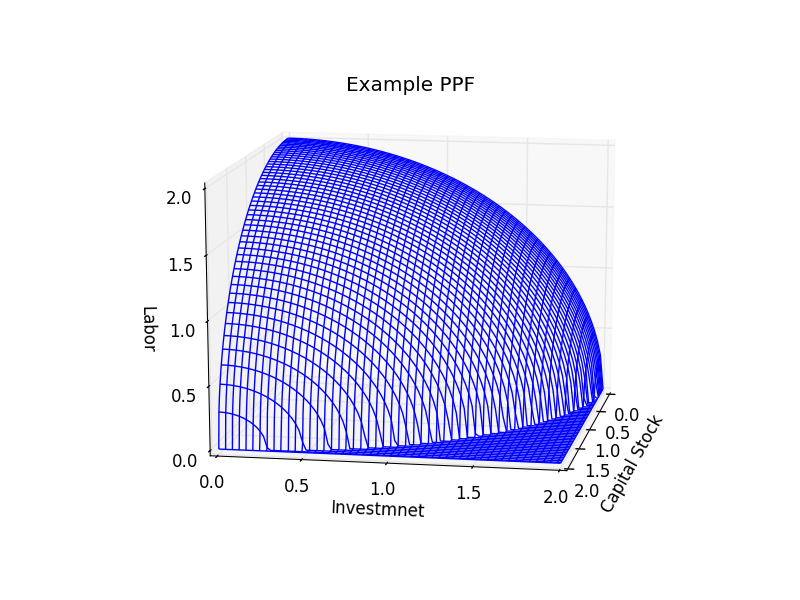
\includegraphics[scale=.31]{example_ppf_wire.png}
    \label{fig:ppf}
  \end{center}

  Second maximization.  Consumer chooses $L_t$

  \begin{align}
    \max_{L_t} & \ \ \  u[T(k_t, x_t, L_t)] \\
    s.t. \ \ \ & L_t \geq 0
  \end{align}

  yielding a period return $V(k_t, x_t) = u[T(k_t, x_t, L(k_t, x_t))]$.  So I think we've ``maximized away'' the labor choice by writing it in terms of $k_t, x_t$.

  finally giving

  \begin{align}
    \max_{k_{t=0}^\infty} & \ \ \ \sum_{t=0}^{\infty} \delta^t V(k_t, k_{t+1} - \beta k_t)\\
    s.t. \ \ \ & \beta k_t + \bar{x}_{k_t} \geq k_{t+1} \geq \beta k_t
  \end{align}

  Which is similar to condition \ref{eq:24_7_profit} above.
  
  
\subsection{Seed No Labor}
\label{sub:seed_no_labor}
  
  No labor, so like the first model, but we let $\beta < 1$. We get a value function:

  \begin{equation} \label{eq:no_labor_vf}
    v(k) = \max u(c) + \delta v((\beta + \zeta)k - \beta c)\\
  \end{equation}
  
  Substitute in:

  \begin{equation}
      v(k) = \max u(\frac{(\beta + \zeta)k - k'}{\beta}) + \delta v((\beta + \zeta)k - \beta c  
  \end{equation}  
  Giving first order condition on consumption, the envelope condition, and the Euler equation:

  \begin{align}
<<<<<<< HEAD
    &\frac{u'(c)}{\beta} = \delta v'(k') \label{no_labor_foc}\\
    &\frac{(\beta + \zeta)}{\beta} u'(c) = v'(k) \label{no_labor_ec} \\
    &\frac{u'(c)}{u'(c')} = \delta(\beta + \zeta) \label{no_labor_ee}
=======
  \end{align}

\subsection{Seed 24/7 With Labor}
\label{sub:seed_24_7_with_labor}

  Including labor again with only one type of output, capital growing exogenously (given $k_0$) at $\beta^t$.  They start with a Leontieff production function so in equilibrium when $c_t = k_t = L_t$.  Again we have that competitive rents of (marginal utility - marginal cost) --- that is ($u'(c_t) - w$)--- accrue to the innovator.  These drop to zero as the total supply grows.  Scarcity of supply is driving this all again.
\subsection{Seed Spillovers and Externalities}
\label{sub:seed_spillovers_and_externalities}

\subsection{Seed-Pills and Reverse Engineering}
\label{sub:seed_pills_and_reverse_engineering}

\section{TODO}
\label{sec:todo}

  \begin{itemize}
    \item Figure out model 1: Seed with 24/7.
    \item Cross partial on $T_{l_t,x_t}$. Done
    \item Resource constraint in 2.2.1 $k = c + \frac{x}{\beta}$ Probably done.
  \end{itemize}
  
\bibliographystyle{apa}
\bibliography{citations}
\label{bib:bibliography}

\end{document}  
